\chapter{ذوبان الأجسام الصلبة الأيونية والجزيئية}\label{ch:g11:dissolution}

رشة ملح تُحرَّك في الماء تختفي في ثوانٍ؛ والرشة نفسها تُحرَّك في زيت الطهي
فتبقى في قاع الكأس، دون تغيير، ما شاء أحد أن يراقبها. والمقلاة الدهنية التي
تُشطف تحت الصنبور تبقى دهنية؛ فإذا أُضيفت قطرة من سائل غسل الأطباق انفصل الدهن.
فما الذي يقرر هل تذوب مادة في سائل؟ يكمن الجواب في الشحنات الجزئية والقوى بين
الجسيمات التي رأيناها في الفصل السابق.

\begin{recall}
\omterm{def:g6:solutions-and-solubility:solubility}{الذوبانية}؛ والسوائل القابلة للامتزاج وغير القابلة له
(\cref{ch:g6:solutions-and-solubility}). \omterm{def:g9:ions:ionic-compound}{والمركب الأيوني} مكوّن من كاتيونات
وأنيونات بنسب تجعله متعادلًا (\cref{ch:g9:ions}). \omterm{def:g7:atoms-and-molecules:molecule}{والجزيئات} القطبية وغير
القطبية، والروابط الهيدروجينية، وتآثرات فان دير فالس
(\cref{ch:g11:polarity-and-cohesion}). \omterm{def:g10:chemical-species:extraction}{والاستخلاص سائل--سائل}
(\cref{ch:g10:chemical-species}). \omterm{def:g10:concentration-and-dilution:molar-concentration}{والتركيز المولي}
(\cref{ch:g10:concentration-and-dilution}).
\end{recall}

\section{ذوبان جسم صلب أيوني}

في بلورة كلوريد الصوديوم يحيط بكل \omterm{def:g9:ions:ion}{أيون} صوديوم \ce{Na+} \omterm{def:g9:ions:ion}{أيونات} كلوريد \ce{Cl-}
ويحيط بكل \omterm{def:g9:ions:ion}{أيون} كلوريد \omterm{def:g9:ions:ion}{أيونات} صوديوم، ويمسكها كلها التجاذب بين الشحنات المتعاكسة.
\omterm{def:g7:atoms-and-molecules:molecule}{وجزيئات} الماء، وهي قطبية، تجذبها هذه الشحنات: فيتجه جانبها الأكسجيني
($\delta^-$) نحو الكاتيونات، وجانبها الهيدروجيني ($\delta^+$) نحو الأنيونات.

\begin{definition}[التفكك]\label{def:g11:dissolution:dissociation}
\emph{تفكك}\index{تفكك} جسم صلب أيوني في \omterm{def:g6:solutions-and-solubility:solute}{مذيب} هو انفصال أيوناته بعضها عن
بعض: فهي تغادر البلورة وتتباعد في \omterm{def:g2:mixing-and-dissolving:dissolve}{المحلول}.
\end{definition}

\begin{definition}[الذوبنة والإماهة]\label{def:g11:dissolution:solvation}
\emph{ذوبنة}\index{ذوبنة} جسيم ذائب هي إحاطته \omterm{def:g7:atoms-and-molecules:molecule}{بجزيئات} \omterm{def:g6:solutions-and-solubility:solute}{المذيب}، التي يمسكها به
التجاذب؛ وتسمى في الماء \emph{الإماهة}\index{إماهة}. والرمز (aq) بعد الصيغة
يعني «مُماه».
\end{definition}

\begin{proposition}[مراحل الذوبان الثلاث]\label{prop:g11:dissolution:stages}
\omterm{def:g2:mixing-and-dissolving:dissolve}{يذوب} الجسم الصلب الأيوني في الماء في ثلاث مراحل تحدث معًا: تُنتزع \omterm{def:g9:ions:ion}{الأيونات} من
البلورة (\omterm{def:g11:dissolution:dissociation}{التفكك})، وتحيط بها \omterm{def:g7:atoms-and-molecules:molecule}{جزيئات} الماء (\omterm{def:g11:dissolution:solvation}{الإماهة})، وتنتشر في \omterm{def:g2:mixing-and-dissolving:dissolve}{المحلول} كله
(التشتت). ولكلوريد الصوديوم،
\[
  \ce{NaCl(s) -> Na+(aq) + Cl-(aq)} .
\]
\end{proposition}

\begin{proof}
نقبله: فالتجاذبات بين \omterm{def:g9:ions:ion}{الأيونات} \omterm{def:g7:atoms-and-molecules:molecule}{وجزيئات} الماء القطبية، إذا جُمعت، تكون من القوة
بحيث تحل محل التجاذبات بين \omterm{def:g9:ions:ion}{أيونات} البلورة.
\end{proof}

\begin{omfigure}
\begin{tikzpicture}[font=\small]
  % the crystal edge: alternating ions
  \foreach \i in {0,1,2,3,4} \foreach \j in {0,1,2,3} {
    \pgfmathtruncatemacro\k{mod(\i+\j,2)}
    \ifnum\k=0
      \node[om atom, ball color=green!60!black, minimum size=6.4mm] at (0.8*\i,0.8*\j) {};
    \else
      \node[om atom, ball color=violet!70, minimum size=4.0mm] at (0.8*\i,0.8*\j) {};
    \fi
  }
  % a hydrated Na+ that has left: O towards the ion
  \begin{scope}[shift={(5.6,1.8)}]
    \node[om atom, ball color=violet!70, minimum size=4.0mm] (na) at (0,0) {};
    \node[font=\footnotesize] at (0,0) {};
    \foreach \a in {0,90,180,270} {
      \node[aO, minimum size=4.6mm] (o\a) at (\a:0.62) {};
      \node[aH, minimum size=3.2mm] (ha\a) at ($(\a:0.62)+(\a+52:0.42)$) {};
      \node[aH, minimum size=3.2mm] (hb\a) at ($(\a:0.62)+(\a-52:0.42)$) {};
      \begin{scope}[on background layer]
        \draw[bond, line width=1.2pt] (o\a.center) -- (ha\a.center);
        \draw[bond, line width=1.2pt] (o\a.center) -- (hb\a.center);
      \end{scope}
    }
    \node[anchor=north] at (0,-1.35) {\ce{Na+(aq)}};
  \end{scope}
  % a hydrated Cl- that has left: H towards the ion
  \begin{scope}[shift={(8.6,1.4)}]
    \node[om atom, ball color=green!60!black, minimum size=6.4mm] at (0,0) {};
    \foreach \a in {45,135,225,315} {
      \node[aH, minimum size=3.2mm] (h\a) at (\a:0.62) {};
      \node[aO, minimum size=4.6mm] (o\a) at (\a:1.0) {};
      \node[aH, minimum size=3.2mm] (k\a) at ($(\a:1.0)+(\a+75:0.42)$) {};
      \begin{scope}[on background layer]
        \draw[bond, line width=1.2pt] (o\a.center) -- (h\a.center);
        \draw[bond, line width=1.2pt] (o\a.center) -- (k\a.center);
      \end{scope}
    }
    \node[anchor=north] at (0,-1.45) {\ce{Cl-(aq)}};
  \end{scope}
  \node[anchor=north, align=center] at (1.6,-0.45) {البلورة\\
    (\foreignlanguage{arabic}{\ce{Na+} صغير، \ce{Cl-} كبير})};
\end{tikzpicture}

{\small \omterm{def:g2:mixing-and-dissolving:dissolve}{ذوبان} كلوريد الصوديوم. غادر \omterm{def:g9:ions:ion}{أيون} صوديوم \omterm{def:g9:ions:ion}{وأيون} كلوريد البلورة؛ وكل منهما
مُماه. حول \omterm{def:g9:ions:ion}{الكاتيون} توجّه \omterm{def:g7:atoms-and-molecules:molecule}{جزيئات} الماء \omterm{def:g7:atoms-and-molecules:atom}{ذرات} أكسجينها (الحمراء، $\delta^-$) نحو
الداخل، وحول \omterm{def:g9:ions:ion}{الأنيون} \omterm{def:g7:atoms-and-molecules:atom}{ذرات} هيدروجينها (البيضاء،
$\delta^+$).}
\end{omfigure}

\section{تراكيز الأيونات}

\begin{method}[تركيز كل أيون]\label{met:g11:dissolution:ions}
\begin{enumerate}
  \item اكتب معادلة \omterm{def:g2:mixing-and-dissolving:dissolve}{الذوبان}، موزونة في \omterm{def:g7:atoms-and-molecules:atom}{الذرات} وفي الشحنة:
        لكلوريد الكالسيوم، \ce{CaCl2(s) -> Ca^{2+}(aq) + 2Cl-(aq)}.
  \item احسب \omterm{def:g10:the-mole:amount}{كمية مادة} الجسم الصلب \omterm{def:g6:solutions-and-solubility:solute}{المذاب} $n$، وتركيز \omterm{def:g2:mixing-and-dissolving:dissolve}{المحلول}
        من \omterm{def:g6:solutions-and-solubility:solute}{المذاب} $c = n / V$.
  \item تركيز كل \omterm{def:g9:ions:ion}{أيون} هو التركيز $c$ مضروبًا في معامله
        في المعادلة: وهنا $[\ce{Ca^{2+}}] = c$
        و$[\ce{Cl-}] = 2c$.
\end{enumerate}
ويدل المعقوفان $[\ldots]$ على \omterm{def:g10:concentration-and-dilution:molar-concentration}{التركيز المولي} لنوع
ذائب.
\end{method}

\begin{example}[كلوريد الكالسيوم]\label{ex:g11:dissolution:cacl2}
% ledger: aw:Ca, aw:Cl
تُذاب \qty{5.55}{g} من كلوريد الكالسيوم ($M = \qty{111.1}{g/mol}$)
لتحضير \qty{500.0}{mL} من \omterm{def:g2:mixing-and-dissolving:dissolve}{المحلول}: $n = \qty{0.0500}{mol}$،
و$c = \qty{0.100}{mol/L}$، إذن $[\ce{Ca^{2+}}] = \qty{0.100}{mol/L}$
و$[\ce{Cl-}] = \qty{0.200}{mol/L}$. والمحلول متعادل: $2 \times
0.100$ من الشحنة الموجبة في اللتر مقابل $1 \times 0.200$ من السالبة.
\end{example}

\section{القطبية والذوبانية}

\begin{proposition}[الشبيه يذيب شبيهه]\label{prop:g11:dissolution:like}
\omterm{def:g6:solutions-and-solubility:solute}{المذيب} القطبي، مثل الماء، يذيب الأجسام الصلبة الأيونية والأنواع القطبية، ولا
سيما القادرة على تكوين روابط هيدروجينية معه؛ \omterm{def:g6:solutions-and-solubility:solute}{والمذيب} غير القطبي، مثل الهكسان
الحلقي أو زيت نباتي، يذيب الأنواع غير القطبية. أما الأجسام الصلبة الأيونية
فتذوب قليلًا جدًا في المذيبات غير القطبية، والأنواع غير القطبية قليلًا جدًا في
الماء.
\end{proposition}

\begin{proof}
نقبله: \omterm{def:g6:solutions-and-solubility:solute}{فالمذاب} \omterm{def:g2:mixing-and-dissolving:dissolve}{يذوب} جيدًا حين تكون التجاذبات التي يستطيع تكوينها مع \omterm{def:g6:solutions-and-solubility:solute}{المذيب} في قوة
التجاذبات التي يكسرها على الأقل، بين جسيماته هو وبين \omterm{def:g7:atoms-and-molecules:molecule}{جزيئات}
\omterm{def:g6:solutions-and-solubility:solute}{المذيب}.
\end{proof}

\begin{example}[ثلاث حالات]\label{ex:g11:dissolution:cases}
% ledger: sol:I2-water, sol:I2-heptane
يمتزج الإيثانول بالماء بكل النسب: فمجموعته \ce{O-H} تكوّن روابط هيدروجينية مع
الماء. \omterm{def:g2:mixing-and-dissolving:dissolve}{ويذوب} الملح في الماء لا في الزيت. واليود، \ce{I2}، وهو \omterm{def:g11:polarity-and-cohesion:polar-molecule}{جزيء غير قطبي}،
\omterm{def:g2:mixing-and-dissolving:dissolve}{يذوب} قليلًا في الماء (نحو \qty{0.3}{g/L}، \omterm{def:g2:mixing-and-dissolving:dissolve}{محلول} بني) لكنه \omterm{def:g2:mixing-and-dissolving:dissolve}{يذوب} جيدًا في
المذيبات غير القطبية (\qty{17}{g} في كيلوغرام الهبتان، \omterm{def:g2:mixing-and-dissolving:dissolve}{محلول}
بنفسجي).
\end{example}

\section{الاستخلاص سائل--سائل، مشروحًا}

ينقل \omterm{def:g10:chemical-species:extraction}{الاستخلاص سائل--سائل} نوعًا من \omterm{def:g6:solutions-and-solubility:solute}{مذيب} إلى \omterm{def:g6:solutions-and-solubility:solute}{مذيب} آخر، \omterm{def:g6:solutions-and-solubility:miscible}{غير قابل للامتزاج}
بالأول، \omterm{def:g2:mixing-and-dissolving:dissolve}{يذوب} فيه النوع أكثر. والقاعدة «الشبيه يذيب شبيهه» تدل على \omterm{def:g6:solutions-and-solubility:solute}{المذيب}
الواجب اختياره.

\begin{inthelab}[استخلاص اليود]
يُصب \qty{20}{mL} من \omterm{def:g2:mixing-and-dissolving:dissolve}{محلول} اليود المائي البني في قمع فصل مع
\qty{10}{mL} من الهكسان الحلقي. يُسدّ القمع، ويُرج، ويُخفَّف ضغطه عبر الصنبور،
ثم يُترك ساكنًا. فتتكوّن طبقتان: الهكسان الحلقي، الأقل كثافة، في الأعلى. وتصير
الطبقة العليا بنفسجية، والسفلى شبه عديمة اللون: فقد انتقل اليود إلى الهكسان
الحلقي. وتُصرَّف الطبقة السفلى عبر الصنبور، ويُستعاد اليود في الهكسان
الحلقي.
\end{inthelab}

\begin{omfigure}
\begin{tikzpicture}[font=\small, scale=1.15]
  \pic[transform shape] at (0,0) {sepfunnel={orange!55!brown!70}{white}};
  \node[anchor=north, align=center] at (0,-0.15) {قبل الرج};
  \draw[omProp, <-] (0.55,2.1) -- (1.4,2.5) node[right, text=black] {الهكسان الحلقي};
  \draw[omProp, <-] (0.45,1.35) -- (1.4,1.2) node[right, text=black,
    align=left] {يود مائي\\ (بني)};
  \pic[transform shape] at (4.6,0) {sepfunnel={orange!10}{violet!60}};
  \node[anchor=north, align=center] at (4.6,-0.15) {بعد الرج\\ والترك};
  \draw[omProp, <-] (5.15,2.1) -- (6.0,2.5) node[right, text=black,
    align=left] {يود في\\ الهكسان الحلقي (بنفسجي)};
  \draw[omProp, <-] (5.05,1.35) -- (6.0,1.2) node[right, text=black,
    align=left] {ماء، شبه\\ عديم اللون};
\end{tikzpicture}

{\small \omterm{def:g10:chemical-species:extraction}{استخلاص} اليود من الماء بالهكسان الحلقي. ينتقل اليود غير القطبي إلى \omterm{def:g6:solutions-and-solubility:solute}{المذيب}
غير القطبي؛ والهكسان الحلقي، الأقل كثافة من الماء، يطفو في
الأعلى.}
\end{omfigure}

\begin{safety}{\ghs[0.82cm]{GHS02}\ghs[0.82cm]{GHS07}\ghs[0.82cm]{GHS08}\ghs[0.82cm]{GHS09}}
% ledger: ghs:I2, ghs:cyclohexane
الهكسان الحلقي شديد القابلية للاشتعال، وبخاره يسبب النعاس، وهو ضار بالرئتين إذا
ابتُلع وشديد السمية للأحياء المائية. واليود ضار بملامسة الجلد وإذا استُنشق. ساحبة
الغازات، ونظارات واقية وقفازات، ولا لهب في الجوار أبدًا؛ وتُجمع النفايات
العضوية.
\end{safety}


\section{الصابون والجزيئات المحبة للوسطين}

\begin{definition}[المحب للماء والكاره للماء]\label{def:g11:dissolution:hydrophilic}
يكون نوع أو جزء من \omterm{def:g7:atoms-and-molecules:molecule}{جزيء} \emph{محبًا للماء}\index{محب للماء}
إذا جذبه الماء (مجموعات أيونية أو قطبية، أو مجموعات تكوّن روابط هيدروجينية)؛
ويكون \emph{كارهًا للماء}\index{كاره للماء} إذا لم يجذبه
(سلاسل طويلة من \omterm{def:g7:atoms-and-molecules:atom}{ذرات} الكربون والهيدروجين، غير قطبية). والأنواع الكارهة للماء
تذوب في الدهون والزيوت.
\end{definition}

\begin{definition}[الجزيء المحب للوسطين والمذيلة]\label{def:g11:dissolution:amphiphilic}
\omterm{def:g7:atoms-and-molecules:molecule}{الجزيء} أو \omterm{def:g9:ions:ion}{الأيون} \emph{المحب للوسطين}\index{محب للوسطين} له رأس \omterm{def:g11:dissolution:hydrophilic}{محب للماء}
وذيل \omterm{def:g11:dissolution:hydrophilic}{كاره للماء}. وفي الماء تتجمع \omterm{def:g9:ions:ion}{الأيونات} المحبة للوسطين في
\emph{مذيلات}\index{مذيلة}: كريات دقيقة ذيولها في الداخل، بعيدًا عن الماء،
ورؤوسها على السطح، ملامسة له.
\end{definition}

\begin{example}[صابون]\label{ex:g11:dissolution:soap}
% ledger: aw:C, aw:H, aw:O, aw:Na
ستيارات الصوديوم، \ce{C17H35COONa} ($M = \qty{306.0}{g/mol}$)، صابون
نموذجي، يُصنع من الدهون الحيوانية أو النباتية. \omterm{def:g2:mixing-and-dissolving:dissolve}{ويذوب} في الماء أيوناتِ صوديوم
\ce{Na+} وأيوناتِ ستيارات \ce{C17H35COO-}: رأسها
\ce{-COO-}، أيوني، \omterm{def:g11:dissolution:hydrophilic}{محب للماء}، وذيلها من 17 \omterm{def:g7:atoms-and-molecules:atom}{ذرة} كربون،
\omterm{def:g11:dissolution:hydrophilic}{كاره للماء}.
\end{example}

\begin{omfigure}
\begin{tikzpicture}[font=\small]
  % the stearate ion as a zigzag of 17 carbons + COO-
  \foreach \k in {0,1,2,3,4,5,6,7,8,9,10,11,12,13,14,15,16} {
    \pgfmathsetmacro\y{mod(\k,2)==0 ? 0 : 0.3}
    \coordinate (c\k) at (0.42*\k,\y);
  }
  \draw[line width=0.9pt] (c0) \foreach \k in {1,2,3,4,5,6,7,8,9,10,11,12,13,14,15,16} { -- (c\k) };
  \coordinate (cc) at ($(c16)+(30:0.42)$);
  \begin{scope}[on background layer]
    \fill[omDef!15, rounded corners] ($(cc)+(-0.25,-0.55)$) rectangle ($(cc)+(1.05,0.9)$);
  \end{scope}
  \draw[line width=0.9pt] (c16) -- (cc);
  \draw[line width=0.9pt] (cc) -- ++(90:0.4) node[above] {O};
  \draw[line width=0.9pt] ([xshift=1.5pt]cc) -- ++(90:0.36);
  \draw[line width=0.9pt] (cc) -- ++(-30:0.42) node[right] {O$^-$};
  \draw[omProp] ($(c0)+(0,-0.15)$) -- ++(0,-0.15) -- ($(c16)+(0,-0.3)$) -- ++(0,0.15);
  \node[omProp, anchor=north] at ($(c8)+(0,-0.32)$) {ذيل كاره للماء (17 ذرة كربون)};
  \node[omDef, anchor=south] at ($(cc)+(0.35,0.9)$) {رأس محب للماء};
  % the sketch
  \begin{scope}[yshift=-1.9cm]
    \draw[omProp, line width=1.6pt, decorate, decoration={snake, amplitude=1.5pt,
      segment length=6pt}] (2.0,0) -- (5.2,0);
    \fill[omDef] (5.45,0) circle (0.25);
    \node[white, font=\scriptsize\bfseries] at (5.45,0) {$-$};
    \node[anchor=west] at (5.9,0) {الأيون نفسه، مرسومًا مبسَّطًا};
  \end{scope}
\end{tikzpicture}

{\small \omterm{def:g9:ions:ion}{أيون} الستيارات. في هذا الرسم المتعرج كل زاوية من السلسلة \omterm{def:g7:atoms-and-molecules:atom}{ذرة} كربون تحمل
\omterm{def:g7:atoms-and-molecules:atom}{ذرات} هيدروجين (\ce{CH2}، و\ce{CH3} في الطرف البعيد)؛ ويشرح فصل لاحق هذا
الاختصار. وفي الأسفل الرسم المبسَّط المعتاد: ذيل متموج ورأس
مستدير.}
\end{omfigure}

\begin{proposition}[كيف يزيل الصابون الدهن]\label{prop:g11:dissolution:soap}
الدهن \omterm{def:g11:dissolution:hydrophilic}{كاره للماء} ولا \omterm{def:g2:mixing-and-dissolving:dissolve}{يذوب} فيه. وفي الماء المصبَّن تذوب ذيول \omterm{def:g9:ions:ion}{أيونات} الصابون في الدهن
بينما تبقى الرؤوس في الماء؛ فيتكسر الدهن قطيرات دقيقة، تلتف كل منها في \omterm{def:g11:dissolution:amphiphilic}{مذيلة}
يواجه سطحها المشحون الماء، ويحمل ماء الشطف القطيرات
بعيدًا.
\end{proposition}

\begin{proof}
نقبله: فهو ينتج عن قاعدة «الشبيه يذيب شبيهه» مطبقةً على كل طرف من طرفي
\omterm{def:g9:ions:ion}{الأيون}؛ والرؤوس المشحونة في الخارج تمنع أيضًا القطيرات من الاندماج من جديد، لأن
الشحنات المتماثلة تتنافر.
\end{proof}

\begin{omfigure}
\begin{tikzpicture}[font=\small]
  \fill[yellow!45!orange!35] (0,0) circle (1.0);
  \node at (0,0) {دهن};
  \foreach \a in {0,20,40,60,80,100,120,140,160,180,200,220,240,260,280,300,320,340} {
    \draw[omProp, line width=1.3pt, decorate, decoration={snake,
      amplitude=1pt, segment length=4pt}] (\a:0.55) -- (\a:1.45);
    \fill[omDef] (\a:1.6) circle (0.15);
  }
  \node[anchor=west, align=left] at (2.4,0.6) {\foreignlanguage{arabic}{الرؤوس \babelsublr{($-$)} في الماء}};
  \node[anchor=west, align=left] at (2.4,-0.4) {الذيول في الدهن};
  \draw[black!50] (2.4,0.6) -- (1.75,0.45);
  \draw[black!50] (2.4,-0.4) -- (1.05,-0.25);
  \node[font=\small, blue!50!black] at (-2.6,1.4) {ماء};
\end{tikzpicture}

{\small \omterm{def:g11:dissolution:amphiphilic}{مذيلة} في مقطع عرضي: \omterm{def:g9:ions:ion}{أيونات} صابون حول قطيرة دهن، ذيولها نحو الداخل،
ورؤوسها المشحونة نحو الخارج. وكل \omterm{def:g11:dissolution:amphiphilic}{مذيلة} مشحونة سلبيًا على سطحها، \omterm{def:g11:dissolution:amphiphilic}{والمذيلات}
يتنافر بعضها مع بعض.}
\end{omfigure}

\begin{omfigure}
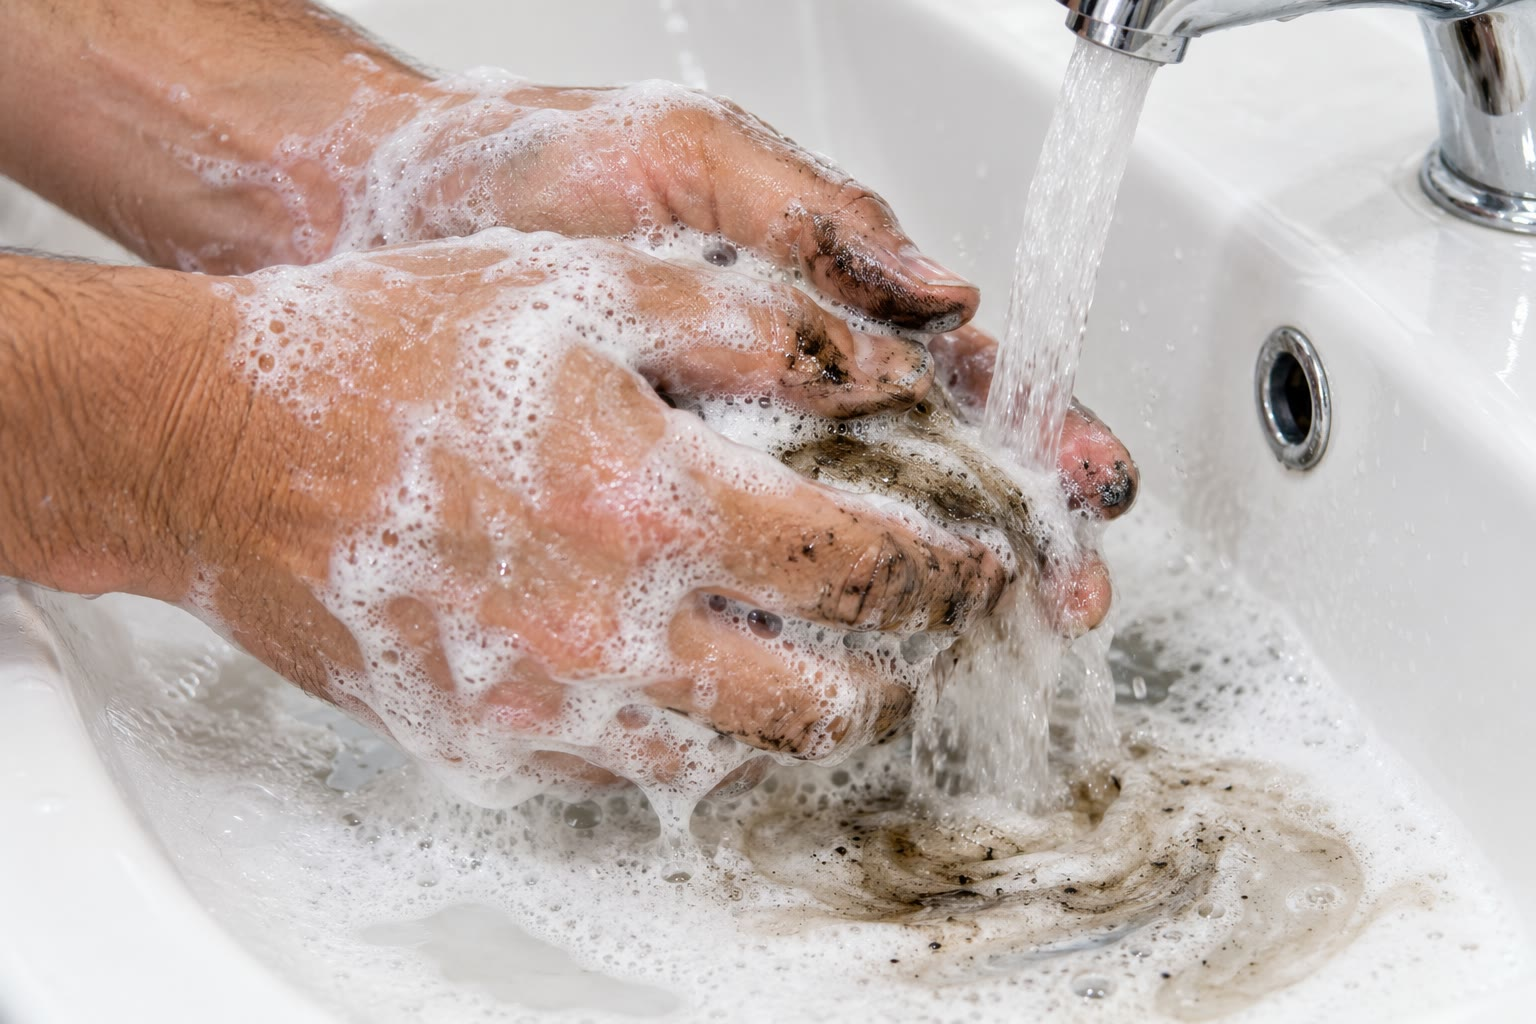
\includegraphics[width=0.48\linewidth]{images/book1/ai/g11-greasy-hands.jpg}

{\small غسل اليدين الدهنيتين: يحمل الصابون الدهن في \omterm{def:g11:dissolution:amphiphilic}{مذيلات}.}
\end{omfigure}

\begin{remark}[الماء العسر والزَّبَد]\label{rem:g11:dissolution:scum}
الماء العسر يحوي كثيرًا من \omterm{def:g9:ions:ion}{أيونات} الكالسيوم \ce{Ca^{2+}} \omterm{def:g9:ions:ion}{وأيونات} المغنيسيوم
\ce{Mg^{2+}}، المذابة من الصخور التي جرى فيها. ومع \omterm{def:g9:ions:ion}{أيونات} الستيارات تكوّن راسبًا
(\cref{ch:g9:ions})، هو ستيارات الكالسيوم:
\[
  \ce{2C17H35COO- + Ca^{2+} -> Ca(C17H35COO)2(s)} .
\]
وهذا الجسم الصلب الرمادي هو الزبد الذي يطوّق المغسلة، وكل \omterm{def:g9:ions:ion}{أيون} صابون يُحتجز فيه
يضيع على الغسل: ففي الماء العسر يرغي الصابون رغوة رديئة حتى تُضاف منه كمية تكفي
لترسيب الكالسيوم كله.
\end{remark}

\begin{omfigure}
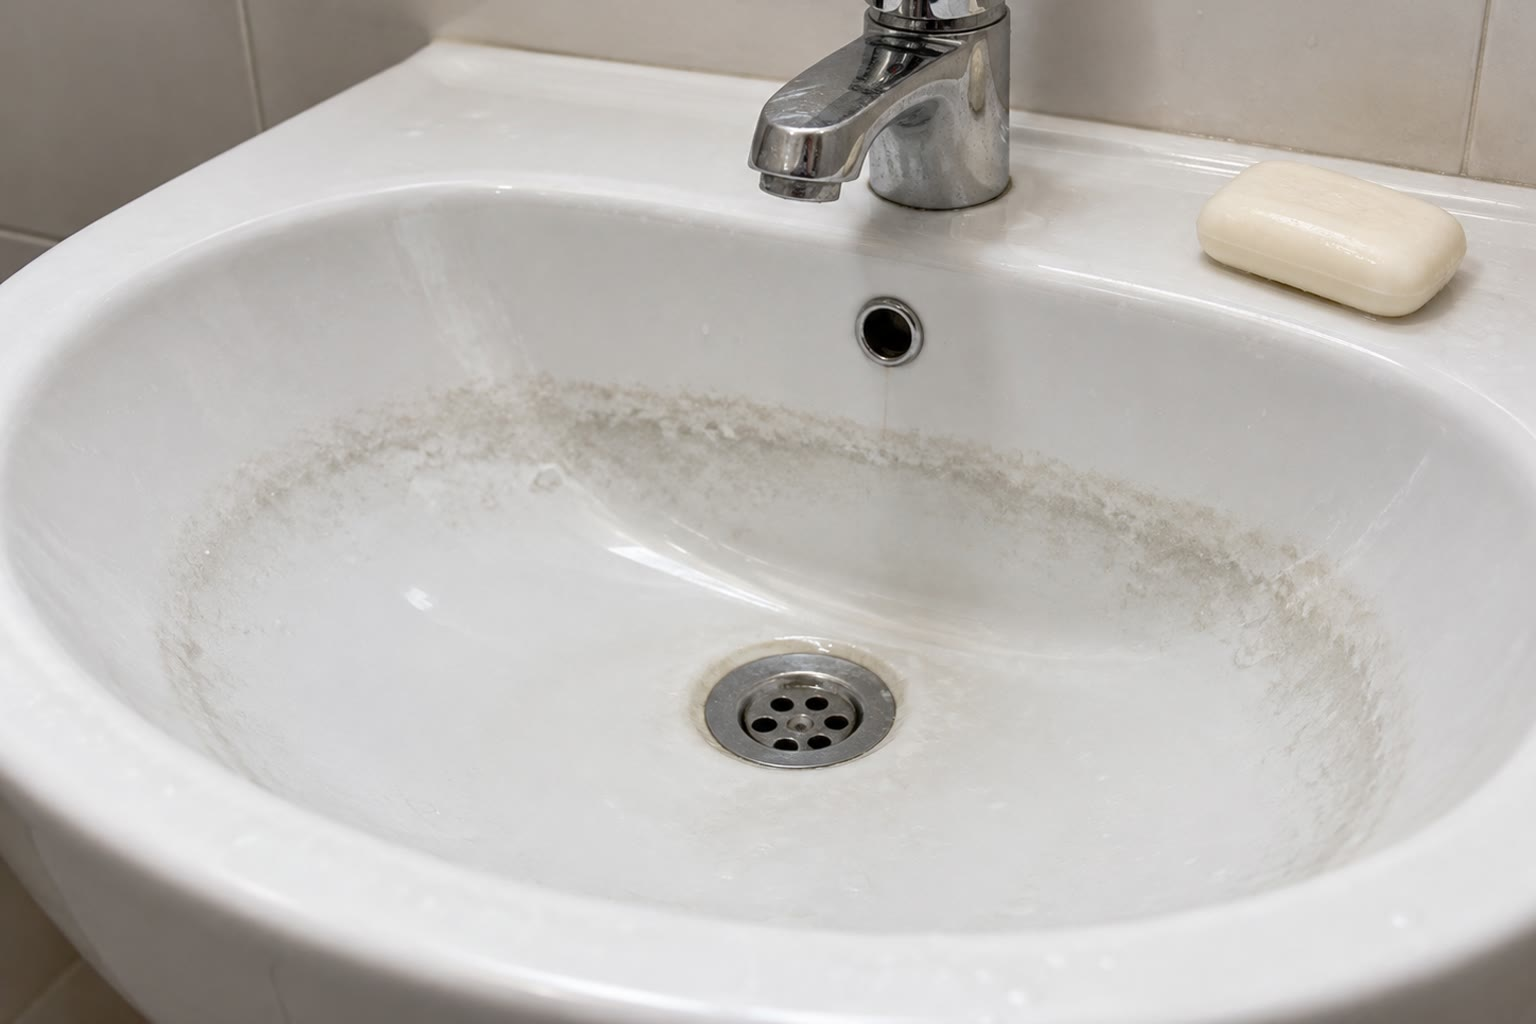
\includegraphics[width=0.45\linewidth]{images/book1/ai/g11-soap-scum.jpg}

{\small زبد الصابون في مغسلة: ستيارات الكالسيوم، رسّبها الماء
العسر.}
\end{omfigure}

\section{تمارين}


\begin{exercise}[$\star$]\label{exo:g11:dissolution:1}
اكتب معادلات \omterm{def:g2:mixing-and-dissolving:dissolve}{ذوبان} كلوريد الصوديوم \ce{NaCl}، وكلوريد الكالسيوم \ce{CaCl2}،
وكبريتات الصوديوم \ce{Na2SO4}، وكلوريد الألومنيوم
\ce{AlCl3} في الماء.
\end{exercise}

\begin{exercise}[$\star$]\label{exo:g11:dissolution:2}
\omterm{def:g2:mixing-and-dissolving:dissolve}{محلول} من كبريتات الصوديوم فيه $c = \qty{0.050}{mol/L}$. أعطِ
تركيزي \omterm{def:g9:ions:ion}{أيونات} الصوديوم \omterm{def:g9:ions:ion}{وأيونات} الكبريتات.
\end{exercise}

\begin{exercise}[$\star$]\label{exo:g11:dissolution:3}
ما المقصود \omterm{def:g11:dissolution:solvation}{بإماهة} \omterm{def:g9:ions:ion}{الأيون}؟ وأي طرف من \omterm{def:g7:atoms-and-molecules:molecule}{جزيء} الماء يتجه نحو \omterm{def:g9:ions:ion}{الكاتيون}، وأيهما نحو
\omterm{def:g9:ions:ion}{الأنيون}؟ ولماذا؟
\end{exercise}

\begin{exercise}[$\star$]\label{exo:g11:dissolution:4}
تُذاب \qty{2.67}{g} من كلوريد الألومنيوم لتحضير
\qty{200.0}{mL} من \omterm{def:g2:mixing-and-dissolving:dissolve}{المحلول}. احسب تركيز \omterm{def:g2:mixing-and-dissolving:dissolve}{المحلول}
وتركيز كل \omterm{def:g9:ions:ion}{أيون}.
\end{exercise}

\begin{exercise}[$\star$]\label{exo:g11:dissolution:5}
صنّف كل جزء من \omterm{def:g9:ions:ion}{أيون} الستيارات على أنه \omterm{def:g11:dissolution:hydrophilic}{محب للماء} أو \omterm{def:g11:dissolution:hydrophilic}{كاره للماء}، وقل
لماذا.
\end{exercise}

\begin{exercise}[$\star\star$]\label{exo:g11:dissolution:6}
أي المذيبين، الماء أم الهكسان الحلقي، تختار لإذابة: الملح؛ وشمع الشموع (سلاسل
هيدروكربونية طويلة)؛ والسكر (مجموعات \ce{O-H} كثيرة)؛ واليود؟ علّل كل
اختيار.
\end{exercise}

\begin{exercise}[$\star\star$]\label{exo:g11:dissolution:7}
يمتزج الإيثانول \ce{CH3-CH2-OH} بالماء بكل النسب، أما الهكسان
\ce{C6H14} فلا يمتزج بالماء. علّل.
\end{exercise}

\begin{exercise}[$\star\star$]\label{exo:g11:dissolution:8}
انظر إلى شكل \omterm{def:g11:dissolution:amphiphilic}{المذيلة}. لماذا تكون الذيول في الداخل والرؤوس في الخارج؟ ولماذا لا
تندمج مذيلتان في قطرة دهن أكبر؟
\end{exercise}

\begin{exercise}[$\star\star$]\label{exo:g11:dissolution:9}
عطر نباتي \omterm{def:g6:solutions-and-solubility:solute}{مذاب} في الماء. لاستخلاصه يستطيع كيميائي أن يستعمل الإيثانول أو الهكسان
الحلقي. أيهما المناسب، ولماذا لا يناسب الآخر (فكّر في
قابلية الامتزاج)؟
\end{exercise}

\begin{exercise}[$\star\star$]\label{exo:g11:dissolution:10}
في \omterm{def:g10:chemical-species:extraction}{استخلاص} اليود، لماذا تكون طبقة الهكسان الحلقي في الأعلى؟ وأي طبقة تُصرَّف عبر
الصنبور؟ وأين يكون اليود في النهاية؟
\end{exercise}

\begin{exercise}[$\star\star$]\label{exo:g11:dissolution:11}
يُرج \omterm{def:g2:mixing-and-dissolving:dissolve}{محلول} أزرق من كبريتات النحاس مع الهكسان الحلقي. ماذا يحدث للون الأزرق؟
علّل.
\end{exercise}

\begin{exercise}[$\star\star\star$]\label{exo:g11:dissolution:12}
ما كتلة كلوريد الكالسيوم الواجب إذابتها لتحضير \qty{250.0}{mL}
من \omterm{def:g2:mixing-and-dissolving:dissolve}{محلول} فيه $[\ce{Cl-}] = \qty{0.300}{mol/L}$؟
\end{exercise}

\begin{exercise}[$\star\star\star$]\label{exo:g11:dissolution:13}
وُجد أن عيّنة من ماء البحر تحوي \qty{0.010}{mol/L} من \omterm{def:g9:ions:ion}{أيونات} الكالسيوم
و\qty{0.053}{mol/L} من \omterm{def:g9:ions:ion}{أيونات} المغنيسيوم. اشرح لماذا يرغي الصابون العادي
رغوة رديئة جدًا في ماء البحر. وما كمية ستيارات الصوديوم التي ترسّبها \omterm{def:g9:ions:ion}{أيونات}
الكالسيوم وحدها في لتر واحد من ماء البحر؟
\end{exercise}

\begin{exercise}[$\star\star\star$]\label{exo:g11:dissolution:14}
يُخلط \qty{100.0}{mL} من \omterm{def:g2:mixing-and-dissolving:dissolve}{محلول} كلوريد الصوديوم تركيزه \qty{0.20}{mol/L}
مع \qty{100.0}{mL} من \omterm{def:g2:mixing-and-dissolving:dissolve}{محلول} كلوريد الكالسيوم تركيزه
\qty{0.10}{mol/L}. ولا يتكوّن \omterm{def:g9:ions:precipitate}{راسب}. احسب تراكيز
\ce{Na+} و\ce{Ca^{2+}} و\ce{Cl-} في \omterm{def:g6:pure-substances-and-mixtures:mixture}{الخليط}، وتحقق من أنه
متعادل.
\end{exercise}

\begin{exercise}[$\star\star\star$]\label{exo:g11:dissolution:15}
% ledger: sol:I2-water, sol:I2-heptane, rho:heptane
\omterm{def:g2:mixing-and-dissolving:dissolve}{يذوب} اليود بنحو \qty{0.3}{g} في لتر الماء
و\qty{17}{g} في كيلوغرام الهبتان. وكثافة الهبتان نحو
\qty{0.68}{kg/L}. كم مرة يزيد ما يحمله لتر من الهبتان من اليود على ما يحمله
لتر من الماء؟ وماذا يعني ذلك \omterm{def:g10:chemical-species:extraction}{للاستخلاص}؟
\end{exercise}

\section{مسألة: الصابون والماء العسر}

\begin{problem}[{مسألة نهاية الأسبوع --- كم من الصابون يضيّع حمام من الماء
العسر زبدًا؟}]
\label{pb:g11:dissolution:1}
% ledger: aw:Ca, aw:Mg, aw:C, aw:H, aw:O, aw:Na
ماء صنبور يحوي \qty{120}{mg} من \omterm{def:g9:ions:ion}{أيونات} الكالسيوم و\qty{24}{mg} من
\omterm{def:g9:ions:ion}{أيونات} المغنيسيوم في اللتر. يُملأ حوض استحمام بحجم \qty{150}{L} منه، ويستعمل
المستحم صابونًا من ستيارات الصوديوم، \ce{C17H35COONa}.

\medskip
\noindent\textbf{الجزء الأول --- ما في الماء.}
\begin{enumerate}
  \item من أين تأتي \omterm{def:g9:ions:ion}{أيونات} الكالسيوم والمغنيسيوم في ماء الصنبور؟
  \item احسب التركيزين الموليين \omterm{def:g9:ions:ion}{لأيونات} الكالسيوم ولأيونات
        المغنيسيوم.
  \item تصحب \omterm{def:g9:ions:ion}{أيونات} الكالسيوم \omterm{def:g9:ions:ion}{أيونات} هيدروجين الكربونات،
        \ce{HCO3-}، كأن هيدروجين كربونات الكالسيوم \ce{Ca(HCO3)2} قد
        أُذيب. اكتب معادلة \omterm{def:g2:mixing-and-dissolving:dissolve}{الذوبان} تلك، واستنتج
        تركيز \omterm{def:g9:ions:ion}{أيونات} هيدروجين الكربونات المرافقة
        للكالسيوم.
  \item ما كمية \omterm{def:g9:ions:ion}{أيونات} الكالسيوم في الحوض؟
\end{enumerate}

\medskip
\noindent\textbf{الجزء الثاني --- الصابون.}
\begin{enumerate}[resume]
  \item احسب \omterm{def:g10:the-mole:molar-mass}{الكتلة المولية} لستيارات الصوديوم.
  \item اكتب معادلة ذوبانه في الماء.
  \item أي جزء من \omterm{def:g9:ions:ion}{أيون} الستيارات \omterm{def:g11:dissolution:hydrophilic}{محب للماء}، وأيهما
        \omterm{def:g11:dissolution:hydrophilic}{كاره للماء}؟ ولماذا يُسمى محبًا للوسطين؟
  \item صف \omterm{def:g11:dissolution:amphiphilic}{المذيلة}، واشرح كيف تزيل الدهن عن
        الجلد.
  \item لماذا يجب أن يُذاب الصابون في الماء، لا في الزيت، للغسل؟
\end{enumerate}

\medskip
\noindent\textbf{الجزء الثالث --- الزبد.}
\begin{enumerate}[resume]
  \item اكتب معادلة ترسيب ستيارات الكالسيوم.
        وتحقق من أنها موزونة في الشحنة.
  \item املأ \omterm{def:g10:reaction-progress-table:extent}{جدول التقدّم} لحجم \qty{1.00}{L} من ماء الصنبور
        ولأيونات ستيارات بزيادة. أي المتفاعلين محدِّد؟
  \item ما كمية \omterm{def:g9:ions:ion}{أيونات} الستيارات التي تضيع في كل لتر بسبب الكالسيوم؟
  \item احسب \omterm{def:g10:the-mole:molar-mass}{الكتلة المولية} لستيارات الكالسيوم، وكتلة الزبد
        المتكوّن في كل لتر.
  \item تترسب ستيارات المغنيسيوم بالطريقة نفسها. ما كمية
        الستيارات التي تأخذها \omterm{def:g9:ions:ion}{أيونات} المغنيسيوم في كل لتر؟
\end{enumerate}

\medskip
\noindent\textbf{الجزء الرابع --- الحوض.}
\begin{enumerate}[resume]
  \item ما كمية \omterm{def:g9:ions:ion}{أيونات} الستيارات التي يرسّبها كالسيوم الحوض
        كله؟
  \item ما كتلة الصابون التي يمثلها ذلك؟
  \item بإضافة المغنيسيوم، ما الكتلة الكلية للصابون الضائع؟
  \item يزن قالب الصابون نحو \qty{100}{g}. كم قالبًا يأخذ
        الكالسيوم وحده؟
  \item اذكر الجواب النهائي: ما كتلة الصابون التي يضيّعها كالسيوم حوض واحد
        من \qty{150}{L} من هذا الماء زبدًا؟
\end{enumerate}
\end{problem}
